\documentclass{beamer}
\usepackage[english,russian]{babel}
\usepackage[utf8]{inputenc}
\usepackage{amsmath}
\usepackage{hyperref}
\usetheme{Warsaw}
\usepackage{listings}
\usepackage{xcolor}
\usepackage{tikz}
\usetikzlibrary{graphs}
\usepackage{algpseudocode}

\lstset{
    frame=tb,
    tabsize=4,
    showstringspaces=false,
    numbers=left,
    commentstyle=\color{green},
    keywordstyle=\color{blue},
    stringstyle=\color{red},
    emph={baz},
    emphstyle=\textbf
}

\begin{document}

\title{Задачи разрешимости логических формул и приложения\newline Лекция 6. Оптимизации алгоритма Conflict-Driven Clause Learning}
\author{Роман Холин}
\institute{Московский государственный университет}
\date{Москва, 2021}

\begin{frame}
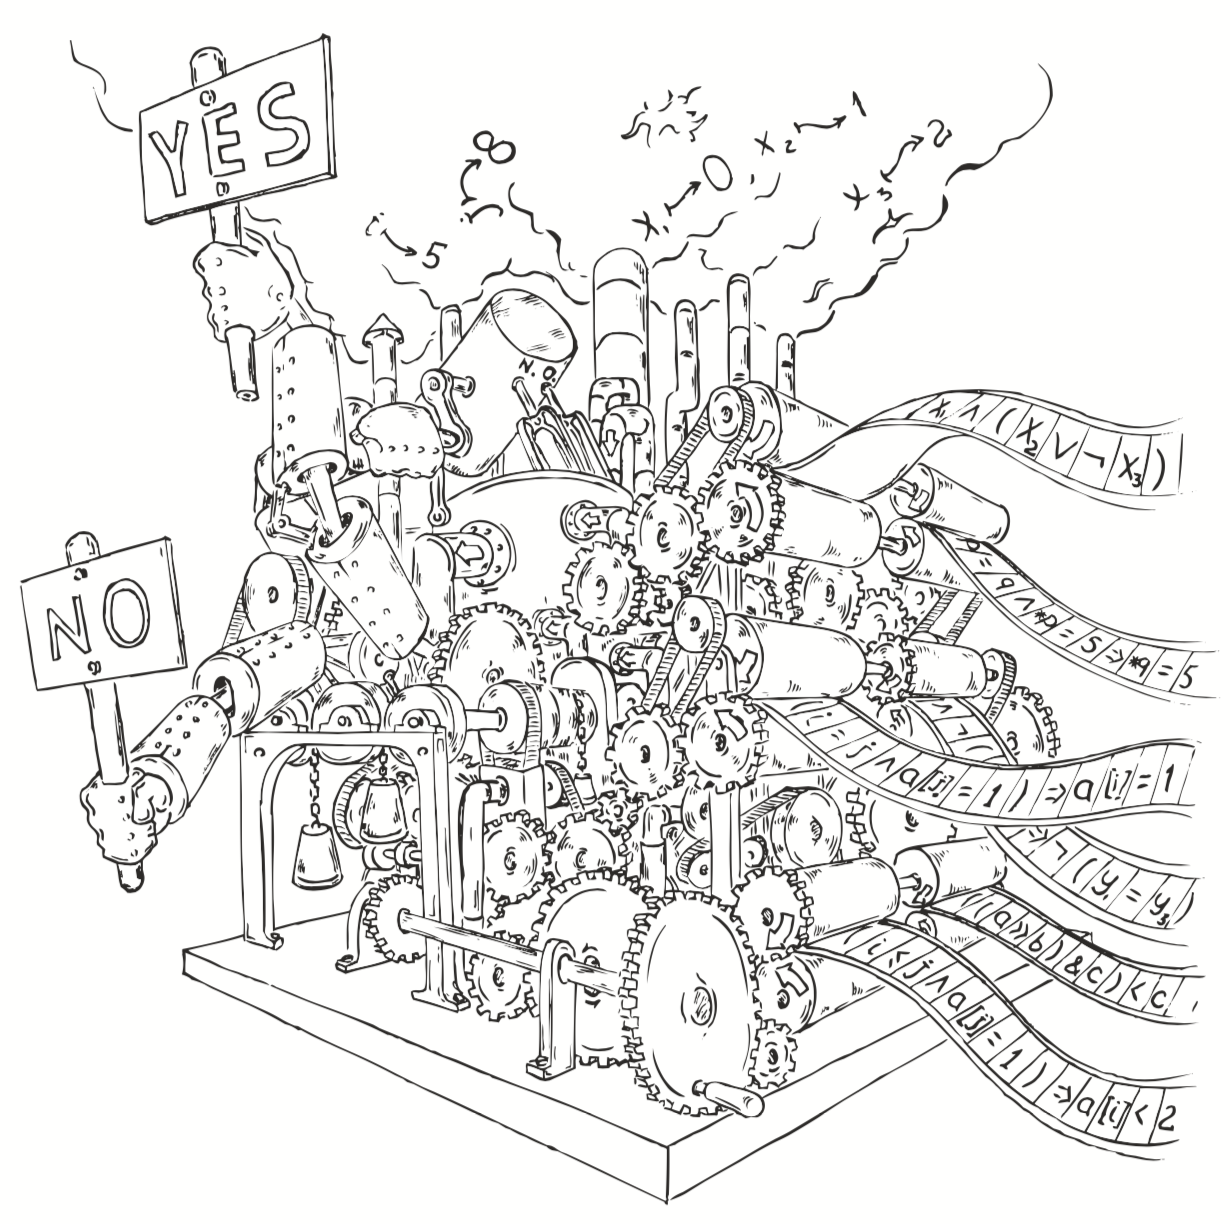
\includegraphics[scale=0.5]{../decision-procedure.png}
\end{frame}

\frame{\titlepage}

\begin{frame}{Conflict-driven clause learning}
\begin{algorithmic}
\Function {CDCL}{}
    \While {true}
        \While {BCP() = "conflict"}
            \State backtrack-level := Analyze-Conflict()
            \If {backtrack-level < 0}
                \State return "Unsatisfiable"
            \EndIf
            \State BackTrack(backtrack-level)
            \If {$\lnot$ Decide()}
                \State return "Satisfiable"
            \EndIf
        \EndWhile
    \EndWhile
\EndFunction
\end{algorithmic}
\end{frame}

\begin{frame}{Граф следствий}
\begin{itemize}
\item Будем писать $x_i@dl$, если на уровне принятия решений dl мы присвоили переменной $x_i$ значение истина и $\lnot x_i@dl$ -
если присволи ложь
\item Вершины графа - переменные, определенные частичной оценкой
\item Из $v_i$ идет ребро $v_j$, если $v_j$ оценена в результате BCP() и $v_i$ входит в дизъюнкт-предпосылку $c$. Эти ребра
помечаются меткой $c$
\item Если есть "конфликт", то ему соответствует вершина. Пусть $c$ - конфликтный дизъюнкт. Тогда к вершине "конфликт" идут
ребра от переменных, входящих в $c$ и они помечаются меткой $c$
\end{itemize}
\end{frame}

\begin{frame}{Пример}
$c_1 = (\lnot x_1 \vee x_2 )$\newline
$c_2 = (\lnot x_1 \vee x_3 \vee x_5 )$\newline
$c_3 = (\lnot x_2 \vee x_4 )$\newline
$c_4 = (\lnot x_3 \vee \lnot x_4 )$\newline
$c_5 = (x_1 \vee x_5 \vee \lnot x_2 )$\newline
$c_6 = (x_2 \vee x_3 )$\newline
$c_7 = (x_2 \vee \lnot x_3 )$\newline
$c_8 = (x_6 \vee \lnot x_5 )$\newline
\end{frame}

\begin{frame}{Пример}
$c_1 = (\lnot x_1 \vee x_2 )$\newline
$c_2 = (\lnot x_1 \vee x_3 \vee x_5 )$\newline
$c_3 = (\lnot x_2 \vee x_4 )$\newline
$c_4 = (\lnot x_3 \vee \lnot x_4 )$\newline
$c_5 = (x_1 \vee x_5 \vee \lnot x_2 )$\newline
$c_6 = (x_2 \vee x_3 )$\newline
$c_7 = (x_2 \vee \lnot x_3 )$\newline
$c_8 = (x_6 \vee \lnot x_5 )$\newline
Пусть $x_1@6$ и $\lnot x_5@3$
\end{frame}

\begin{frame}{Пример}
$c_1 = (\lnot x_1 \vee x_2 )$\newline
$c_2 = (\lnot x_1 \vee x_3 \vee x_5 )$\newline
$c_3 = (\lnot x_2 \vee x_4 )$\newline
$c_4 = (\lnot x_3 \vee \lnot x_4 )$\newline
$c_5 = (x_1 \vee x_5 \vee \lnot x_2 )$\newline
$c_6 = (x_2 \vee x_3 )$\newline
$c_7 = (x_2 \vee \lnot x_3 )$\newline
$c_8 = (x_6 \vee \lnot x_5 )$\newline
Пусть $x_1@6$ и $\lnot x_5@3$\newline
$c_9 = (x_5 \vee \lnot x_1)$\newline
\end{frame}

\begin{frame}{Пример}
$c_1 = (\lnot x_1 \vee x_2 )$\newline
$c_2 = (\lnot x_1 \vee x_3 \vee x_5 )$\newline
$c_3 = (\lnot x_2 \vee x_4 )$\newline
$c_4 = (\lnot x_3 \vee \lnot x_4 )$\newline
$c_5 = (x_1 \vee x_5 \vee \lnot x_2 )$\newline
$c_6 = (x_2 \vee x_3 )$\newline
$c_7 = (x_2 \vee \lnot x_3 )$\newline
$c_8 = (x_6 \vee \lnot x_5 )$\newline
Пусть $x_1@6$ и $\lnot x_5@3$\newline
$c_9 = (x_5 \vee \lnot x_1)$\newline
Откатимся до 3 уровня принятия решений
\end{frame}

\begin{frame}{}
\begin{itemize}
\item Почему откатились на 3 уровень, а не на 5?
\end{itemize}
\end{frame}

\begin{frame}{}
\begin{itemize}
\item Почему откатились на 3 уровень, а не на 5?
\item Эмпирические исследования показывают, что так быстрее
\end{itemize}
\end{frame}

\begin{frame}{}
\begin{itemize}
\item Почему откатились на 3 уровень, а не на 5?
\item Эмпирические исследования показывают, что так быстрее
\item Почему останавливаемся?
\end{itemize}
\end{frame}

\begin{frame}{}
\begin{itemize}
\item Почему откатились на 3 уровень, а не на 5?
\item Эмпирические исследования показывают, что так быстрее
\item Почему останавливаемся?
\item Докажем от противного
\end{itemize}
\end{frame}

\begin{frame}{Бинарная резолюция}
$\begin{array}{rl}
    & (a_1 \vee \dots a_n \vee c) (b_1 \dots b_m \vee \lnot c)\\
    \cline{2-2}
    & (a_1 \vee \dots a_n \vee b_1 \dots b_m)
\end{array}$
\end{frame}

\begin{frame}{Бинарная резолюция}
$\begin{array}{rl}
    & (a_1 \vee \dots a_n \vee c) (b_1 \dots b_m \vee \lnot c)\\
    \cline{2-2}
    & (a_1 \vee \dots a_n \vee b_1 \dots b_m)
\end{array}$\newline
Известен результат, что КНФ не выполнима тогда и только тогда, когда существует конечное число бинарных резолюций, приводящих к
пустому дизъюнкту
\end{frame}

\begin{frame}{Пример}
$c_1 = (\lnot x_4 \vee x_2 \vee x_5)$\newline
$c_2 = (\lnot x_4 \vee x_{10} \vee x_6)$\newline
$c_3 = (\lnot x_5 \vee \lnot x_6 \vee \lnot x_7)$\newline
$c_4 = (\lnot x_6 \vee x_7)$\newline
\end{frame}

\begin{frame}{Пример}
$c_1 = (\lnot x_4 \vee x_2 \vee x_5)$\newline
$c_2 = (\lnot x_4 \vee x_{10} \vee x_6)$\newline
$c_3 = (\lnot x_5 \vee \lnot x_6 \vee \lnot x_7)$\newline
$c_4 = (\lnot x_6 \vee x_7)$\newline
\begin{itemize}
\item Выберем последний оцененый литерал
\item Выберем дизъюнкт предпосылку данного литерала
\item Применим бинарную резолюцию к конфликтному дизъюнкту и дизъюнкту предпосылке через переменную, соответствующей литералу
\end{itemize}
\end{frame}

\begin{frame}{Пример}
$c_1 = (\lnot x_4 \vee x_2 \vee x_5)$\newline
$c_2 = (\lnot x_4 \vee x_{10} \vee x_6)$\newline
$c_3 = (\lnot x_5 \vee \lnot x_6 \vee \lnot x_7)$\newline
$c_4 = (\lnot x_6 \vee x_7)$\newline
\begin{itemize}
\item Выберем последний оцененый литерал
\item Выберем дизъюнкт предпосылку данного литерала
\item Применим бинарную резолюцию к конфликтному дизъюнкту и дизъюнкту предпосылке через переменную, соответствующей литералу
\end{itemize}
Когда остановиться?
\end{frame}

\begin{frame}{Уникальная точка импликации}
\begin{itemize}
\item Уникальная точка импликации - любая вершина импликационного графа, которая не является вершиной <<конфликт>> и которая
находится на каждом пути, ведущему от конкретной корневой вершины к вершине конкретной вершине <<конфликт>> (в теории графов так
же называется доминатором вершины)
\end{itemize}
\end{frame}

\begin{frame}{Уникальная точка импликации}
\begin{itemize}
\item Уникальная точка импликации - любая вершина импликационного графа, которая не является вершиной <<конфликт>> и которая
находится на каждом пути, ведущему от конкретной корневой вершины к вершине конкретной вершине <<конфликт>> (в теории графов так
же называется доминатором вершины)
\item Первая УТИ - ближайшая к конфликтной вершине уникальная точка импликации
\end{itemize}
\end{frame}

\begin{frame}{Уникальная точка импликации}
\begin{itemize}
\item Уникальная точка импликации - любая вершина импликационного графа, которая не является вершиной <<конфликт>> и которая
находится на каждом пути, ведущему от конкретной корневой вершины к вершине конкретной вершине <<конфликт>> (в теории графов так
же называется доминатором вершины)
\item Первая УТИ - ближайшая к конфликтной вершине уникальная точка импликации
\item Эмпирические исследования показывают, что нужно остановится, когда будет добавлена отрицание первой УТИ текущего уровня
принятия решений
\end{itemize}
\end{frame}

\begin{frame}{Анализ конфликта}
\begin{algorithmic}
\If {current-decision-level = 0}
    \State return -1
\EndIf
\State cl := current-conf licting-clause
\While {$\lnot$ Stop-criterion-met(cl)}
    \State lit := Last-assigned-literal(cl)
    \State var := Variable-of-literal(lit)
    \State ante := Antecedent(lit)
    \State cl := Resolve(cl, ante, var)
\EndWhile
\State add-clause-to-database(cl)
\State return clause-asserting-level(cl)
\end{algorithmic}
\end{frame}

\begin{frame}{Conflict-driven clause learning}
\begin{algorithmic}
\Function {CDCL}{}
    \While {true}
        \While {BCP() = "conflict"}
            \State backtrack-level := Analyze-Conflict()
            \If {backtrack-level < 0}
                \State return "Unsatisfiable"
            \EndIf
            \State BackTrack(backtrack-level)
            \If {$\lnot$ Decide()}
                \State return "Satisfiable"
            \EndIf
        \EndWhile
    \EndWhile
\EndFunction
\end{algorithmic}
\end{frame}

\begin{frame}{Эвристика Jeroslow–Wang}
\begin{itemize}
\item Для каждого литерала посчитаем\newline
$J(l) = \Sigma_{w \in B, l \in w}2^{|w|}$
\end{itemize}
\end{frame}

\begin{frame}{Dynamic Largest Individual Sum (DLIS)}
\begin{itemize}
\item Для каждого литерала посчитаем в скольких неразрешенных дизъюнктах он находится
\end{itemize}
\end{frame}

\begin{frame}{Dynamic Largest Individual Sum (DLIS)}
\begin{itemize}
\item Для каждого литерала посчитаем в скольких неразрешенных дизъюнктах он находится
\item Очень дорого
\end{itemize}
\end{frame}

\begin{frame}{Variable State Independent Decaying Sum (VSIDS)}
\begin{itemize}
\item Для каждого литерала посчитаем в скольких неразрешенных дизъюнктах он находится
\item Иногда всё делим на 2
\item При каждом конфликте, увеличиваем на 1 балл литерала
\end{itemize}
\end{frame}

\begin{frame}{Variable State Independent Decaying Sum (VSIDS) в MiniSAT}
\begin{itemize}
\item При каждом конфликте, увеличиваем на балл литерала на Inc
\item Inc сначала 1, затем увеличивается на 1.5 после каждого конфликта
\item Всё делится на $10^{-100}$, если есть балл, выше $10^{100}$
\end{itemize}
\end{frame}

\begin{frame}{Эвристики, основанные на дизъюнктах (Berkmin)}
\begin{itemize}
\item Для каждого литерала и переменной посчитаем в скольких неразрешенных дизъюнктах он находится
\item Иногда оценки переменной делим на 2
\item При каждом конфликте, увеличиваем на 1 балл литерала
\item Каждый конфликтный дизъюнкт помещаем в стек
\item Когда нужно выбрать, какую перпеменную оценить, находим в стеке самый верхний дизъюнкт, который неразрешен, а в нём
выбираем переменную с самой большой оценкой, а затем литерал с самой большой оценкой
\end{itemize}
\end{frame}

\begin{frame}{Эвристики, основанные на дизъюнктах (Clause-Move-To-Front)}
\begin{itemize}
\item То же самое, что и Berkmin
\item Перед новым дизъюнктом кладем $k$ дизъюнктов, которые участвовали в процессе получения нового дизъюнкта в процессе
бинарных резолюций
\end{itemize}
\end{frame}

\begin{frame}{Противоречивые ядра}
\begin{itemize}
\item Противоречивое ядро противоречивой формулы $f$ - подформула формулы $f$, которое является противоречивой.
\item Минимальное противоречивое ядро противоречивой формулы $f$ - противоречивое ядро, такое, что удаление любый дизъюнктов из
этой формулы делает её выполнимой подформулу выполнимой.
\end{itemize}
\end{frame}

\begin{frame}{Граф резолюций}
\begin{itemize}
\item Вершины - дизъюнкты
\item Корни - первоначальные дизъюнкты
\item Есть ребро - если вершина, к которой было проведено ребро, получена в процессе бинарной резолюции через вершину, от
которой было проведено ребро
\end{itemize}
\end{frame}

\begin{frame}{Conflict-driven clause learning}
\begin{algorithmic}
\Function {CDCL}{}
    \While {true}
        \While {BCP() = "conflict"}
            \State backtrack-level := Analyze-Conflict()
            \If {backtrack-level < 0}
                \State return "Unsatisfiable"
            \EndIf
            \State BackTrack(backtrack-level)
            \If {$\lnot$ Decide()}
                \State return "Satisfiable"
            \EndIf
        \EndWhile
    \EndWhile
\EndFunction
\end{algorithmic}
\end{frame}

\begin{frame}{Граф следствий}
\begin{itemize}
\item Будем писать $x_i@dl$, если на уровне принятия решений dl мы присвоили переменной $x_i$ значение истина и $\lnot x_i@dl$ -
если присволи ложь
\item Вершины графа - переменные, определенные частичной оценкой
\item Из $v_i$ идет ребро $v_j$, если $v_j$ оценена в результате BCP() и $v_i$ входит в дизъюнкт-предпосылку $c$. Эти ребра
помечаются меткой $c$
\item Если есть "конфликт", то ему соответствует вершина. Пусть $c$ - конфликтный дизъюнкт. Тогда к вершине "конфликт" идут
ребра от переменных, входящих в $c$ и они помечаются меткой $c$
\end{itemize}
\end{frame}

\begin{frame}{Пример}
$c_1 = (\lnot x_1 \vee x_2 )$\newline
$c_2 = (\lnot x_1 \vee x_3 \vee x_5 )$\newline
$c_3 = (\lnot x_2 \vee x_4 )$\newline
$c_4 = (\lnot x_3 \vee \lnot x_4 )$\newline
$c_5 = (x_1 \vee x_5 \vee \lnot x_2 )$\newline
$c_6 = (x_2 \vee x_3 )$\newline
$c_7 = (x_2 \vee \lnot x_3 )$\newline
$c_8 = (x_6 \vee \lnot x_5 )$\newline
\end{frame}

\begin{frame}{Пример}
$c_1 = (\lnot x_1 \vee x_2 )$\newline
$c_2 = (\lnot x_1 \vee x_3 \vee x_5 )$\newline
$c_3 = (\lnot x_2 \vee x_4 )$\newline
$c_4 = (\lnot x_3 \vee \lnot x_4 )$\newline
$c_5 = (x_1 \vee x_5 \vee \lnot x_2 )$\newline
$c_6 = (x_2 \vee x_3 )$\newline
$c_7 = (x_2 \vee \lnot x_3 )$\newline
$c_8 = (x_6 \vee \lnot x_5 )$\newline
Пусть $x_1@6$ и $\lnot x_5@3$
\end{frame}

\begin{frame}{Пример}
$c_1 = (\lnot x_1 \vee x_2 )$\newline
$c_2 = (\lnot x_1 \vee x_3 \vee x_5 )$\newline
$c_3 = (\lnot x_2 \vee x_4 )$\newline
$c_4 = (\lnot x_3 \vee \lnot x_4 )$\newline
$c_5 = (x_1 \vee x_5 \vee \lnot x_2 )$\newline
$c_6 = (x_2 \vee x_3 )$\newline
$c_7 = (x_2 \vee \lnot x_3 )$\newline
$c_8 = (x_6 \vee \lnot x_5 )$\newline
Пусть $x_1@6$ и $\lnot x_5@3$\newline
$c_9 = (x_5 \vee \lnot x_1)$\newline
\end{frame}

\begin{frame}{Пример}
$c_1 = (\lnot x_1 \vee x_2 )$\newline
$c_2 = (\lnot x_1 \vee x_3 \vee x_5 )$\newline
$c_3 = (\lnot x_2 \vee x_4 )$\newline
$c_4 = (\lnot x_3 \vee \lnot x_4 )$\newline
$c_5 = (x_1 \vee x_5 \vee \lnot x_2 )$\newline
$c_6 = (x_2 \vee x_3 )$\newline
$c_7 = (x_2 \vee \lnot x_3 )$\newline
$c_8 = (x_6 \vee \lnot x_5 )$\newline
Пусть $x_1@6$ и $\lnot x_5@3$\newline
$c_9 = (x_5 \vee \lnot x_1)$\newline
Откатимся до 3 уровня принятия решений
\end{frame}

\begin{frame}{}
\begin{itemize}
\item Почему откатились на 3 уровень, а не на 5?
\end{itemize}
\end{frame}

\begin{frame}{}
\begin{itemize}
\item Почему откатились на 3 уровень, а не на 5?
\item Эмпирические исследования показывают, что так быстрее
\end{itemize}
\end{frame}

\begin{frame}{}
\begin{itemize}
\item Почему откатились на 3 уровень, а не на 5?
\item Эмпирические исследования показывают, что так быстрее
\item Почему останавливаемся?
\end{itemize}
\end{frame}

\begin{frame}{}
\begin{itemize}
\item Почему откатились на 3 уровень, а не на 5?
\item Эмпирические исследования показывают, что так быстрее
\item Почему останавливаемся?
\item Докажем от противного
\end{itemize}
\end{frame}

\begin{frame}{Бинарная резолюция}
$\begin{array}{rl}
    & (a_1 \vee \dots a_n \vee c) (b_1 \dots b_m \vee \lnot c)\\
    \cline{2-2}
    & (a_1 \vee \dots a_n \vee b_1 \dots b_m)
\end{array}$
\end{frame}

\begin{frame}{Бинарная резолюция}
$\begin{array}{rl}
    & (a_1 \vee \dots a_n \vee c) (b_1 \dots b_m \vee \lnot c)\\
    \cline{2-2}
    & (a_1 \vee \dots a_n \vee b_1 \dots b_m)
\end{array}$\newline
Известен результат, что КНФ не выполнима тогда и только тогда, когда существует конечное число бинарных резолюций, приводящих к
пустому дизъюнкту
\end{frame}

\begin{frame}{Пример}
$c_1 = (\lnot x_4 \vee x_2 \vee x_5)$\newline
$c_2 = (\lnot x_4 \vee x_{10} \vee x_6)$\newline
$c_3 = (\lnot x_5 \vee \lnot x_6 \vee \lnot x_7)$\newline
$c_4 = (\lnot x_6 \vee x_7)$\newline
\end{frame}

\begin{frame}{Пример}
$c_1 = (\lnot x_4 \vee x_2 \vee x_5)$\newline
$c_2 = (\lnot x_4 \vee x_{10} \vee x_6)$\newline
$c_3 = (\lnot x_5 \vee \lnot x_6 \vee \lnot x_7)$\newline
$c_4 = (\lnot x_6 \vee x_7)$\newline
\begin{itemize}
\item Выберем последний оцененый литерал
\item Выберем дизъюнкт предпосылку данного литерала
\item Применим бинарную резолюцию к конфликтному дизъюнкту и дизъюнкту предпосылке через переменную, соответствующей литералу
\end{itemize}
\end{frame}

\begin{frame}{Пример}
$c_1 = (\lnot x_4 \vee x_2 \vee x_5)$\newline
$c_2 = (\lnot x_4 \vee x_{10} \vee x_6)$\newline
$c_3 = (\lnot x_5 \vee \lnot x_6 \vee \lnot x_7)$\newline
$c_4 = (\lnot x_6 \vee x_7)$\newline
\begin{itemize}
\item Выберем последний оцененый литерал
\item Выберем дизъюнкт предпосылку данного литерала
\item Применим бинарную резолюцию к конфликтному дизъюнкту и дизъюнкту предпосылке через переменную, соответствующей литералу
\end{itemize}
Когда остановиться?
\end{frame}

\begin{frame}{Уникальная точка импликации}
\begin{itemize}
\item Уникальная точка импликации - любая вершина импликационного графа, которая не является вершиной <<конфликт>> и которая
находится на каждом пути, ведущему от конкретной корневой вершины к вершине конкретной вершине <<конфликт>> (в теории графов так
же называется доминатором вершины)
\end{itemize}
\end{frame}

\begin{frame}{Уникальная точка импликации}
\begin{itemize}
\item Уникальная точка импликации - любая вершина импликационного графа, которая не является вершиной <<конфликт>> и которая
находится на каждом пути, ведущему от конкретной корневой вершины к вершине конкретной вершине <<конфликт>> (в теории графов так
же называется доминатором вершины)
\item Первая УТИ - ближайшая к конфликтной вершине уникальная точка импликации
\end{itemize}
\end{frame}

\begin{frame}{Уникальная точка импликации}
\begin{itemize}
\item Уникальная точка импликации - любая вершина импликационного графа, которая не является вершиной <<конфликт>> и которая
находится на каждом пути, ведущему от конкретной корневой вершины к вершине конкретной вершине <<конфликт>> (в теории графов так
же называется доминатором вершины)
\item Первая УТИ - ближайшая к конфликтной вершине уникальная точка импликации
\item Эмпирические исследования показывают, что нужно остановится, когда будет добавлена отрицание первой УТИ текущего уровня
принятия решений
\end{itemize}
\end{frame}

\begin{frame}{Анализ конфликта}
\begin{algorithmic}
\If {current-decision-level = 0}
    \State return -1
\EndIf
\State cl := current-conf licting-clause
\While {$\lnot$ Stop-criterion-met(cl)}
    \State lit := Last-assigned-literal(cl)
    \State var := Variable-of-literal(lit)
    \State ante := Antecedent(lit)
    \State cl := Resolve(cl, ante, var)
\EndWhile
\State add-clause-to-database(cl)
\State return clause-asserting-level(cl)
\end{algorithmic}
\end{frame}

\begin{frame}{Conflict-driven clause learning}
\begin{algorithmic}
\Function {CDCL}{}
    \While {true}
        \While {BCP() = "conflict"}
            \State backtrack-level := Analyze-Conflict()
            \If {backtrack-level < 0}
                \State return "Unsatisfiable"
            \EndIf
            \State BackTrack(backtrack-level)
            \If {$\lnot$ Decide()}
                \State return "Satisfiable"
            \EndIf
        \EndWhile
    \EndWhile
\EndFunction
\end{algorithmic}
\end{frame}

\begin{frame}{Эвристика Jeroslow–Wang}
\begin{itemize}
\item Для каждого литерала посчитаем\newline
$J(l) = \Sigma_{w \in B, l \in w}2^{|w|}$
\end{itemize}
\end{frame}

\begin{frame}{Dynamic Largest Individual Sum (DLIS)}
\begin{itemize}
\item Для каждого литерала посчитаем в скольких неразрешенных дизъюнктах он находится
\end{itemize}
\end{frame}

\begin{frame}{Dynamic Largest Individual Sum (DLIS)}
\begin{itemize}
\item Для каждого литерала посчитаем в скольких неразрешенных дизъюнктах он находится
\item Очень дорого
\end{itemize}
\end{frame}

\begin{frame}{Variable State Independent Decaying Sum (VSIDS)}
\begin{itemize}
\item Для каждого литерала посчитаем в скольких неразрешенных дизъюнктах он находится
\item Иногда всё делим на 2
\item При каждом конфликте, увеличиваем на 1 балл литерала
\end{itemize}
\end{frame}

\begin{frame}{Variable State Independent Decaying Sum (VSIDS) в MiniSAT}
\begin{itemize}
\item При каждом конфликте, увеличиваем на балл литерала на Inc
\item Inc сначала 1, затем увеличивается на 1.5 после каждого конфликта
\item Всё делится на $10^{-100}$, если есть балл, выше $10^{100}$
\end{itemize}
\end{frame}

\begin{frame}{Эвристики, основанные на дизъюнктах (Berkmin)}
\begin{itemize}
\item Для каждого литерала и переменной посчитаем в скольких неразрешенных дизъюнктах он находится
\item Иногда оценки переменной делим на 2
\item При каждом конфликте, увеличиваем на 1 балл литерала
\item Каждый конфликтный дизъюнкт помещаем в стек
\item Когда нужно выбрать, какую перпеменную оценить, находим в стеке самый верхний дизъюнкт, который неразрешен, а в нём
выбираем переменную с самой большой оценкой, а затем литерал с самой большой оценкой
\end{itemize}
\end{frame}

\begin{frame}{Эвристики, основанные на дизъюнктах (Clause-Move-To-Front)}
\begin{itemize}
\item То же самое, что и Berkmin
\item Перед новым дизъюнктом кладем $k$ дизъюнктов, которые участвовали в процессе получения нового дизъюнкта в процессе
бинарных резолюций
\end{itemize}
\end{frame}

\begin{frame}{Противоречивые ядра}
\begin{itemize}
\item Противоречивое ядро противоречивой формулы $f$ - подформула формулы $f$, которое является противоречивой.
\item Минимальное противоречивое ядро противоречивой формулы $f$ - противоречивое ядро, такое, что удаление любый дизъюнктов из
этой формулы делает её выполнимой подформулу выполнимой.
\end{itemize}
\end{frame}

\begin{frame}{Граф резолюций}
\begin{itemize}
\item Вершины - дизъюнкты
\item Корни - первоначальные дизъюнкты
\item Есть ребро - если вершина, к которой было проведено ребро, получена в процессе бинарной резолюции через вершину, от
которой было проведено ребро
\end{itemize}
\end{frame}
\begin{frame}
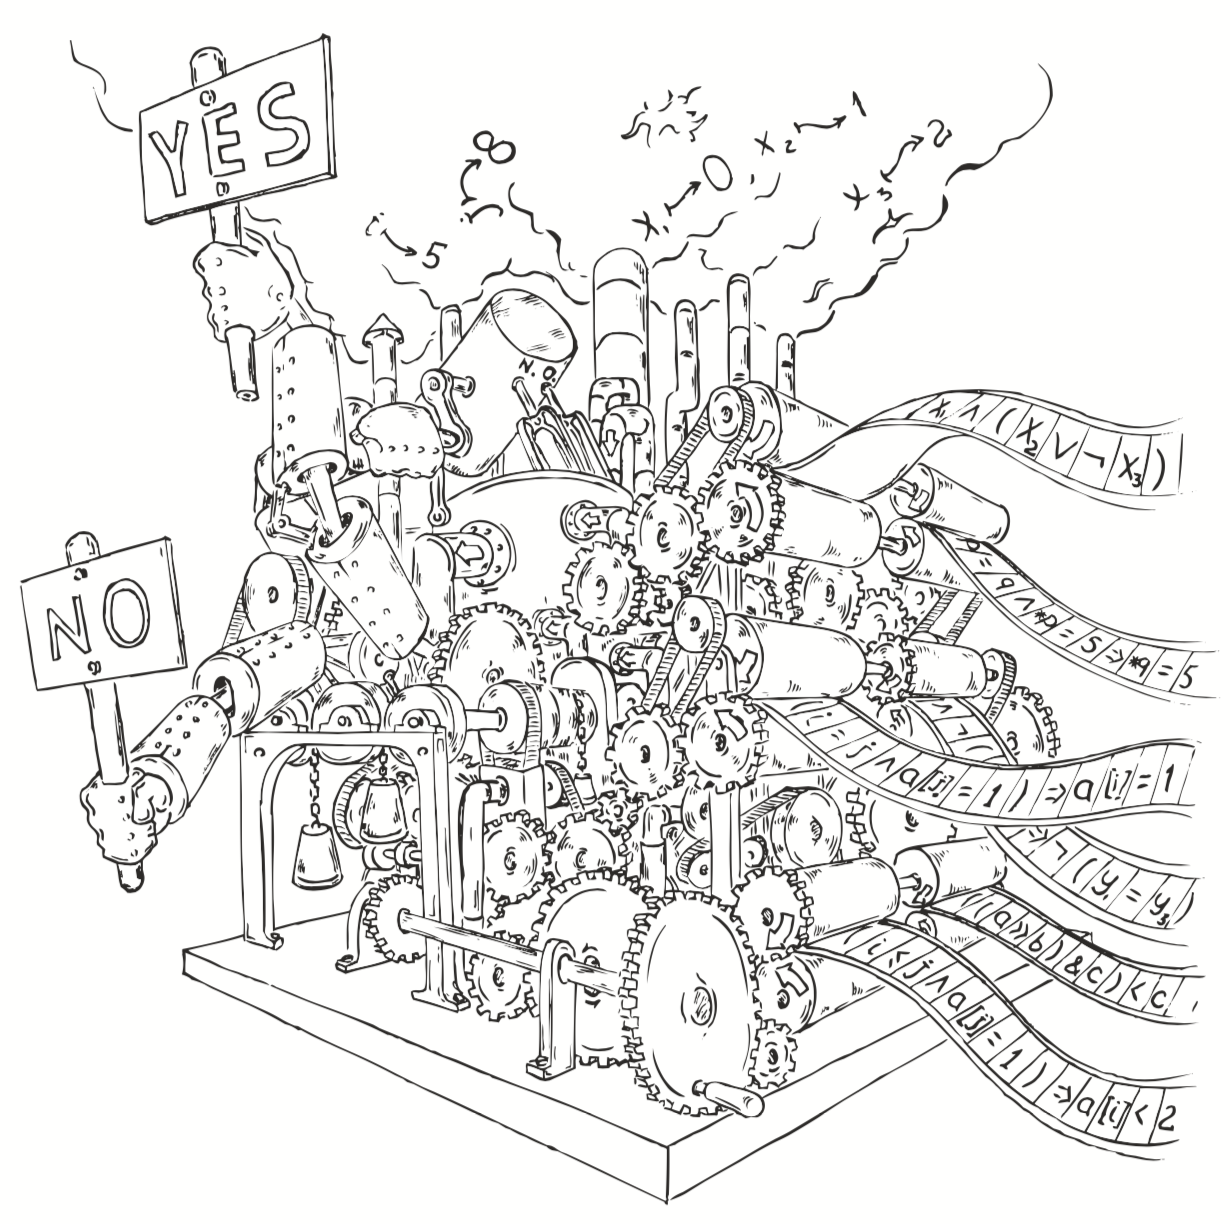
\includegraphics[scale=0.5]{../decision-procedure.png}
\end{frame}

\end{document}
